\section{Discretization of Stokes}
Derive a proper variational formulation of the Stokes problem.
Discuss the four Brezzi conditions that are needed for a well-posed continuous problem.
Explain why oscillations might appear in the pressure for some discretization techniques.
Present expected approximation properties for mixed elements that satisfy the inf-sup condition, and discuss a few examples like e.g.\ Taylor--Hood, Mini, and Crouzeix--Raviart. % chktex 8
Discuss also how one might cirumvent the inf-sup condition by stabilization.

\subsection{Short-form answer}
Stokes problem is given by
\begin{equation}
    \begin{split}
        -\Delta u + \nabla p &= f \quad \text{in } \Omega, \\
        \nabla \cdot u &= 0 \quad \text{in } \Omega, \\
        u &= g \quad \text{on } \partial\Omega_D, \\
        \frac{\partial u}{\partial n} - p\, n &= h \quad \text{on } \partial\Omega_N. \\
    \end{split}
\end{equation}
Here, \( u \colon \Omega \to \mathbb{R}^n \) is the fluid field, while \( p \colon \Omega \to \mathbb{R} \) is the pressure field.
The presence of both the Dirichlet and Neumann boundary conditions leads to a well-posed problem, as long as neither is empty.
If we don't have a Dirichlet boundary, then the velocity field is only determined up to a constant, while if the Neumann boundary is empty, the pressure field is only determined up to a constant.

We find the weak form of the Stokes problem by multiplying the first equation by a test function \( v \in V \) and integrating.
This yields
\begin{align*}
    \int_{\Omega} \left(
        -\Delta u + \nabla p
    \right) \cdot v \diff x &= \int_{\Omega} f \cdot v \diff x, \\
    \int_{\Omega} \nabla u \cdot \nabla v \diff x - \int_\Omega p \nabla \cdot v \diff x &= \int_{\Omega} f \cdot v \diff x + \int_{\partial\Omega} \left(
        \frac{\partial u}{\partial n} - p\, n
    \right) \cdot v \diff s.
\end{align*}
Now applying the boundary conditions, we can split the boundary integral into two parts, one for the Dirichlet boundary and one for the Neumann boundary:
\begin{equation}
    \int_{\partial\Omega} \left(
        \frac{\partial u}{\partial n} - p\, n
    \right) \cdot v \diff s = \int_{\partial\Omega_D} \left(
        \frac{\partial u}{\partial n} - p\, n
    \right) \cdot v \diff s + \int_{\partial\Omega_N} \left(
        \frac{\partial u}{\partial n} - p\, n
    \right) \cdot v \diff s.
\end{equation}
As the solution is known on $\partial\Omega_D$, we can choose $v \in H^1_{0, D}(\Omega)$, such that the first term vanishes.
For the second term, we can simply insert the Neumann condition, which finally gives us
\begin{equation}
    \int_{\Omega} \nabla u \cdot \nabla v \diff x - \int_\Omega p \nabla \cdot v \diff x = \int_{\Omega} f \cdot v \diff x + \int_{\partial\Omega_N} h \cdot v \diff s.
\end{equation}
For the second equation, we multiply by a test function \( q \in Q \) and integrate, which gives us
\begin{equation}
    \int_{\Omega} q \nabla \cdot u \diff x = 0.
\end{equation}
The weak form of the problem is then to find \( (u, p) \in H_{g, D}^1(\Omega) \times L^2(\Omega) \) such that
\begin{equation}
    \begin{split}
        a(u, v) + b(p, v) &= f(v) \quad \forall v \in H_{0,D}^1(\Omega), \\
        b(q, u) &= 0 \:\,\qquad \forall q \in L^2(\Omega).
    \end{split}
\end{equation}
Note that we have here switched \( p := -p \), in order to get symmetry.

For saddle-point problems of the form described, the four Brezzi conditions we need to satisfy is then
\begin{enumerate}
    \item Continuity of $a$: For all \( u_h, v_h \in V_h \), we have
        \begin{equation}
            a(u_h, v_h) \leq C_1 \norm{u_h}_{V_h} \norm{v_h}_{V_h}.
        \end{equation}

    \item Coercivity of $a$: There exists a constant \( C_2 > 0 \) such that
        \begin{equation}
            a(u_h, u_h) \geq C_2 \norm{u_h}_{V_h}^2
        \end{equation}
        for all $u_h \in Z_h$, where
        \begin{equation*}
            Z_h = \{u_h \in V_h \mid b(u_h, q_h) = 0 \quad \forall q_h \in Q_h \}.
        \end{equation*}

    \item Continuity of $b$: For all \( q_h \in Q_h \) and \( u_h \in V_h \), we have
        \begin{equation}
            b(q_h, u_h) \leq C_3 \norm{q_h}_{Q_h} \norm{u_h}_{V_h}.
        \end{equation}

    \item ``Coercivity'' of $b$: There exists a constant \( C_4 > 0 \) such that
        \begin{equation}
            \sup_{u_h \in V_h}\, \frac{b(q_h, u_h)}{\norm{u_h}_{V_h}} \geq C_4 \norm{u_h}_1 \quad \forall q_h \in Q_h.
        \end{equation}
\end{enumerate}
For Stokes problem, the first three conditions aren't too difficult to check.
The last one however is a bit tricky, and typically requires specially designed finite elements in order to satisfy it.

Oscillations appear when the last condition is not satisfied.
This happens because there exists some $q_h \in Q_h$ such that $b(q_h, u_h) = 0$ for all $u_h \in V_h$, while $q_h \neq 0$.
This means that if we have some solution pressure $p_h \in Q_h$, we can simply add as much of $q_h$ as we want.
These spurious pressure modes typically take the form of oscillations.

For mixed elements, we get the expected approximation of
\begin{equation}
    \norm{u - u_h}_{1} + \norm{p - p_h}_{0} \leq C h^k \norm{u}_{k+1} + D h^{t+1} \norm{p}_{t+1},
\end{equation}
where $k$ is the polynomial degree of the velocity space and $t$ is the polynomial degree of the pressure space.

One popular choice of element is the Taylor--Hood element, % chktex 8
which is quadratic in velocity and linear in pressure, while being continuous across element boundaries.
In other words, it's a $P_2$-$P_1$ element.
This gives the expected approximation order of
\begin{equation}
    \norm{u - u_h}_{1} + \norm{p - p_h}_{0} \leq h^2 \left(
        C \norm{u}_{3} + D \norm{p}_{2}
    \right).
\end{equation}
Another popular choice is the mini element, which is linear in both velocity and pressure, however it has an additional bubble function in the velocity.
This bubble function is designed such that it is zero along the element edges, which on the unit triangle means that the basis functions are
\begin{equation}
    \{ 1, x, y, xy(1 - x - y) \},
\end{equation}
where the last function is the bubble function.
This gives the expected approximation order
\begin{equation}
    \norm{u - u_h}_{1} + \norm{p - p_h}_{0} \leq h \left(
        C \norm{u}_{2} + D h \norm{p}_{2}
    \right).
\end{equation}

Finally we have the Crouzeix--Raviart element, % chktex 8
which is linear in velocity and constant in pressure.
Additionally, the velocity is only continuous at the midpoint of each edge,
as illustrated in \cref{fig:crouzeix_raviart}.
With this element, we get the expected approximation order
\begin{equation}
    \norm{u - u_h}_{1} + \norm{p - p_h}_{0} \leq h \left(
        C \norm{u}_{2} + D \norm{p}_{1}
    \right).
\end{equation}

\begin{figure}[htbp]
    \centering
    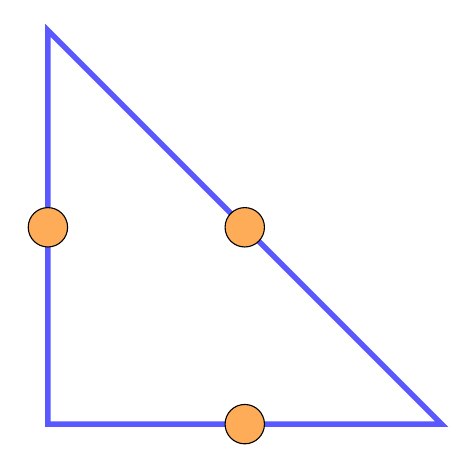
\begin{tikzpicture}[scale=5]
        \draw[line width=2, color=blue!65] (0, 0) -- (1, 0) -- (0, 1) -- cycle;
        \draw[fill=orange!65] (0.5, 0)   circle (0.05);
        \draw[fill=orange!65] (0,   0.5) circle (0.05);
        \draw[fill=orange!65] (0.5, 0.5) circle (0.05);
    \end{tikzpicture}
    \caption{
        Crouzeix--Raviart element with DOFs marked in orange.% chktex 8
        \label{fig:crouzeix_raviart}
    }
\end{figure}

\newpage
\subsection{Long-form answer}
\subsubsection{Weak form of Stokes problem}
The Stokes problem describes the flow of a slowly moving viscous incompressible Newtonian fluid.
Let $u : \Omega \to \mathbb{R}^n$ be the fluid field, and $p: \Omega \to \mathbb{R}$ be the fluid pressure.
Stokes problem can then be written as
\begin{equation}
    \begin{split}
        -\Delta u + \nabla p &= f \quad \text{in } \Omega, \\
        \nabla \cdot u &= 0 \quad \text{in } \Omega, \\
        u &= g \quad \text{on } \partial\Omega_D, \\
        \frac{\partial u}{\partial n} - p \, n &= h \quad \text{on } \partial\Omega_N.
    \end{split}
\end{equation}
Here, $f$ is the body forcce, $\partial\Omega_D$ and $\partial\Omega_N$ are the Dirichlet and Neumann boundaries, respectively.
Additionally, $g$ is the prescribed fluid velocity on the Dirichlet boundary, and $h$ is the surface force or stress on the Neumann boundary.

The presence of the Dirichlet and Neumann boundary conditions lead to a well-posed problem, so long as neither are empty.
If the Dirichlet condition if empty, the velocity is only determined up to a constant.
If the Neumann condition is empty, the pressure is only determined up to a constant.

We being by setting up the weak form of the Stokes problem.
Setting up the weak form amounts to the following steps:
\begin{enumerate}
    \item Multiply by test functions and integrate of the domain $\Omega$.

    \item Integration by parts, and apply Gauss--Green's lemma. % chktex 8

    \item Apply the boundary conditions.
\end{enumerate}
This leads us to initially have, multiplying the first equation by a test function $v$ and the second equation by a test function $q$,
\begin{equation}
    \begin{split}
        \int_\Omega (-\Delta u + \nabla p) \cdot v \, \diff x &= \int_\Omega f \cdot v \, \diff x \\
        \int_\Omega (\nabla \cdot u) q \, \diff x &= 0.
    \end{split}
\end{equation}
This is however not ideal, as we would currently be requiring that $u \in H_{g, D}^2$ and $p \in H^1$.
We therefore apply integration by parts, which yields
\begin{equation}
    \int_\Omega (-\Delta u + \nabla p) \cdot v \, \diff x
    = \int_\Omega \nabla u : \nabla v + p (\nabla \cdot v) \, \diff x
    + \int_{\partial\Omega} \left(\frac{\partial u}{\partial n} - p n\right) \cdot v \, \diff s.
\end{equation}
We then consider the boundary conditions, which yields
\begin{align*}
    \int_{\partial\Omega} \left(\frac{\partial u}{\partial n} - p n\right) \cdot v \, \diff s
    &= {
        \int_{\partial\Omega_D} \left(\frac{\partial u}{\partial n} - p n\right) \cdot v \, \diff s
        + \int_{\partial\Omega_N} \left(\frac{\partial u}{\partial n} - p n\right) \cdot v \, \diff s
    } \\
    &= {
        \underbrace{
            \int_{\partial\Omega_D} \left(\frac{\partial u}{\partial n} - p n\right) \cdot 0 \, \diff s
        }_{\text{As we choose } v \in H^1_{0, D}}
        + \int_{\partial\Omega_N} h \cdot v \, \diff s
    } \\
    &= \int_{\partial\Omega_N} h \cdot v \, \diff s.
\end{align*}
Defining
\begin{equation}
    \begin{split}
        a(u, v) &= \int_{\Omega} \nabla u : \nabla v \, \diff x \\
        b(v, p) &= \int_{\Omega} p (\nabla \cdot v) \, \diff x \\
        L(v) &= \int_{\Omega} f \cdot v \, \diff x + \int_{\partial\Omega_N} h \cdot v \, \diff x
    \end{split}
\end{equation}
we can rewrite the weak form of Stokes problem succinctly as:
Find $(u, p) \in V \times Q$ such that for all $(v, q) \in \hat{V} \times \hat{Q}$
\begin{equation}
    \begin{split}
        a(u, v) - b(v, p) &= L(v), \\
        b(u, q) &= 0.
    \end{split}
\end{equation}

The finite element formulation follows directly from this:
Find $u_h \in V_{g, h}$ and $p_h \in Q_h$ such that
\begin{equation}\label{eq:stokes-fem}
    \begin{split}
        a(u_h, v_h) + b(p_h, v_h) &= L(v_h) \quad \forall v_h \in V_{0, h}, \\
        b(q_h, u_h) &= 0 \quad\qquad \forall q_h \in Q_h.
    \end{split}
\end{equation}

\subsubsection{Brezzi conditions}
For a saddle point problem of the form \cref{eq:stokes-fem} to be well-posed, we require that four conditions are satisfied.
\begin{enumerate}
    \item Boundedness of $a$:
        \begin{equation}
            a(u_h, v_h) \leq C_1 \norm{u_h}_{V_h} \norm{v_{h}}_{V_h}
            \quad
            \forall u_h, v_h \in V_h.
        \end{equation}

    \item Boundedness of $b$:
        \begin{equation}
            b(u_h, q_h) \leq C_2 \norm{u_h}_{V_h} \norm{q_{h}}_{Q_h}
            \quad
            \forall {
                u_h \in V_h,
                q_h \in Q_h.
            }
        \end{equation}

    \item Coersivity of $a$:
        \begin{equation}
            a(u_h, u_h) \geq C_3 \norm{u_h}_{V_h}^2
            \quad
            \forall u_h \in Z_h,
        \end{equation}
        where $Z_h = \{ u_h \in V_h | b(u_h, q_h) = 0 \, \forall q_h \in Q_h \}$.

    \item ``Coercivity'' of $b$:
        \begin{equation}
            \sup_{u_h \in V_h} \frac{
                b(u_h, q_h)
            }{
                \norm{u_h}_{V_h}
            } \geq C_4 \norm{q_h}_{Q_h}
            > 0
            \quad
            \forall q_h \in Q_h.
        \end{equation}
\end{enumerate}
The first three conditions are easily verified for Stokes problem, while the last one is difficult unless the elements are designed specifically to meet this condition.
As the first three a rather simple, they are included here for completeness.

\paragraph{Boundedness of \texorpdfstring{$a$}{a}}
Let $u_h, v_h \in V_h$.
Then we have by the Cauchy--Schwarz inequality % chktex 8
\begin{equation}
    a(u_h, v_h)
    = \int_{\Omega} \nabla u_h : \nabla v_h \, \diff x
    \leq \norm{\nabla u_h}_{L^2} \norm{\nabla v_h}_{L^2}
    \leq \norm{u_h}_1 \norm{v_h}_1.
\end{equation}
This shows that $a$ is bounded, with $C_1 = 1$.

\paragraph{Boundedness of \texorpdfstring{$b$}{b}}
Let $u_h \in V_h$ and $q_h \in Q_h$.
We again utilize Cauchy--Schwarz inequality in order to show the bound, as % chktex 8
\begin{equation}
    b(u_h, q_h)
    = \int_{\Omega} q_h (\nabla \cdot u_h) \, \diff x
    \leq \norm{q_h}_{L^2} \norm{\nabla \cdot u_h}_{L^2}
    \leq \norm{q_h}_{L^2} \norm{u_h}_{1}.
\end{equation}
The tricky portion here is to bound $\norm{\nabla \cdot u_h}_{L^2} \leq \norm{u_h}_{1}$, however we can actually do it without a coefficient, according to Kent.

\paragraph{Coercivity of \texorpdfstring{$a$}{a}}
Finally, let $u_h \in V_h$.
Then, we simply have
\begin{equation}
    a(u_h, u_h)
    = \int_{\Omega} \nabla u_h : \nabla u_h \diff x
    = \norm{\nabla u_h}_{L^2}^2
    \geq C_3 \norm{u_h}_1,
\end{equation}
where we can find $C_3$ as the norms are equivalent on $H^1_0$.

\subsubsection{Oscillations in the pressure}
The simplest case where we discover oscillations in the pressure, is in Poiseuille flow.
The analytical solution here is given by
\begin{equation}
    u = (y(1 - y), 0)
    \quad\text{and}\quad
    p = 1 - x.
\end{equation}
We choose this problem as the solution is known, which simplifies the analysis.

We then discretize the problem in a similarly simple manor, with linear Lagrange elements for velocity and pressure.
What we would see then when we solve the problem is that the velocity is well-represented, while there are wild oscillations present in the pressure.
If we had chosen quadratic elements in the velocity however, both the velocity and the pressure would be captured accurately.

The reason for the appearance of the oscillations with the $P_1$--$P_1$ elements stems from the fact that they are not \textit{inf-sup} stable.
That is, they do not fulfill the fourth Brezzi condition.
The $P_{2}$--$P_{1}$ elements however fulfill this, resulting in a nice solution.

\subsubsection{inf-sup and approximation}
In order to obtain order optimal convergence rates, we require that the $\inf$-$\sup$ condition,
\begin{equation}
    \inf_{p \in Q_h} \sup_{v \in V_{h, g}} \frac{(p, \nabla \cdot v)}{\norm{v}_1 \norm{p}_0}
    \geq \beta
    > 0,
\end{equation}
is satisfied.
When this is satisfied, we get convergence
\begin{equation}
    \norm{u - u_h}_1 + \norm{p - p_h}_0
    \leq C h^k \norm{u}_{k+1} + D h^{\ell + 1} \norm{p}_{\ell + 1},
\end{equation}
where $k$ and $\ell$ are the polynomial degree of the velocity and pressure respectively.
Let's see how this is reflected in the approximations of a couple elements.

\paragraph{The Taylor--Hood element} % chktex 8
For the Taylor--Hood element, we have $u \in P_2$ and $p \in P_1$, subject to the restriction that they are continuous across elements. % chktex 8
This element satisfies the $\inf$-$\sup$ condition, and we can therefore directly get the approximation property
\begin{equation}
    \norm{u - u_h}_1 + \norm{p - p_h}_0
    \leq C h^2 (\norm{u}_3 + \norm{p}_2).
\end{equation}
For the generalized $P_{k}$--$P_{k-1}$ Taylor--Hood element, we similarly get % chktex 8
\begin{equation}
    \norm{u - u_h}_1 + \norm{p - p_h}_0
    \leq C h^k (\norm{u}_{k+1} + \norm{p}_k).
\end{equation}

\paragraph{The Crouzeix--Raviart element} % chktex 8
The Crouzeix--Raviart element also satisfies the $\inf$-$\sup$ condition, and are given by $u \in P_1$ and $p \in P_0$. % chktex 8
Here, $u$ is \emph{only} continuous in the mid-point of each side, and $p$ is discontinuous.
We then get the error estimate
\begin{equation}
    \norm{u - u_h}_1 + \norm{p - p_h}_0
    \leq C h (\norm{u}_2 + \norm{p}).
\end{equation}
It is $\inf$-$\sup$ stable with our formulation of Stokes problem, however if we replace it with the more physically correct formulation
\begin{equation}
    -\nabla \cdot \epsilon(u) - \nabla p = f,
\end{equation}
where $\epsilon(u) = \frac{1}{2} (\nabla + \nabla^T)$ is the symmetric gradient, it cannot be used.
We can generalize the element to odd degrees, but not even.

\paragraph{The Mini element}
The Mini element is linear in velocity and pressure, however it contains an extra degree of freedom in the velocity which is zero on all edges, dubbed a bubble function.
For instance in the 2D case, the bubble function, on the reference triangle, is given by
\begin{equation}
    b(x, y) = xy(1 - x - y).
\end{equation}
This yields the error estimate
\begin{equation}
    \norm{u - u_h}_1 + \norm{p - p_h}_0
    \leq
    C_0 h \norm{u}_2 + C_1 h^2 \norm{p}_2.
\end{equation}
Note that the convergence in the velocity is linear, meaning that adding the bubble function brought stability, but not an increase in approximation order.

\subsubsection{Stability without inf-sup}
When stabilizing, we typically replace a system of the form
\begin{equation}
    \begin{split}
        Au + B^T p &= f \\
        B u &= 0,
    \end{split}
\end{equation}
with a system
\begin{equation}
    \begin{split}
        Au + B^T p &= f \\
        B u - \epsilon Dp &= \epsilon d,
    \end{split}
\end{equation}
where $D$ is a positive, but not necessarily positive definite, matrix.
We obtain a nonsingular system, as multiplying the first equation by $A^{-1}$ and factoring yields
\begin{equation}
    \begin{split}
        u + A^{-1} B^T p &= A^{-1} f \\
        \underbrace{B u}_{\text{Insert second equation}} &= B A^{-1} f - B A^{-1} B^T p \\
        \epsilon d + \epsilon D p &= B A^{-1} f - B A^{-1} B^T p \\
        (B A^{-1} B^T + \epsilon D)p &= BA^{-1} f - \epsilon d,
    \end{split}
\end{equation}
and $(B A^{-1} B^T + \epsilon D)$ is nonsingular if $D$ is nonsingular, as both components are positive.

Solving for $p$ in the second equation we get
\begin{equation}
    \begin{split}
        \epsilon D p &= Bu - \epsilon d \\
        p &= (\epsilon D)^{-1} (Bu - \epsilon d),
    \end{split}
\end{equation}
and inserting this into the second equation yields
\begin{equation}
    \begin{split}
        Au + B^T (\epsilon D)^{-1} (Bu - \epsilon d) &= f \\
        \left( A + \frac{1}{\epsilon} B^T D^{-1} B \right) u &= f + D^{-1} d.
    \end{split}
\end{equation}
Then, $\left( A + \frac{1}{\epsilon} B^T D^{-1} B \right)$ is nonsingular as $A$ is invertible, and $B^T D^{-1} B$ is positive.

The question is then how to choose $D$, and we have a couple of options.
The three main techiques are:
\begin{enumerate}
    \item
        Pressure stabilization, by choosing $\nabla \cdot v + \epsilon \Delta p = 0$.
        This is motivated through the convection-diffusion equation.
        This sets $D = A$.

    \item
        Penalty method, by choosing $\nabla \cdot v + \epsilon p = 0$.
        Typically one then chooses the Velocity-Schur complement.
        This sets $D = M$.

    \item
        Artificial compressibility, by choosing $\nabla \cdot -\epsilon \frac{\partial p}{\partial t}$.
        This is practical as it allows for time stepping.
        This sets $D = \frac{1}{\Delta t} M$.
\end{enumerate}